% LTeX: language=it

\documentclass{../.common/high-school-notebook}

\usetikzlibrary{calc,patterns,angles,quotes}

\hypersetup{
  pdftitle={Quaderno delle regole - Matematica},
  pdfauthor={Tommaso Bocchietti},
  pdfsubject={High School Notebook},
}


\begin{document}
\graphicspath{{../.common/}}

\title{Quaderno delle regole - Matematica}
\author{Tommaso Bocchietti}

\maketitle

\begin{figure}[H]
  \centering
  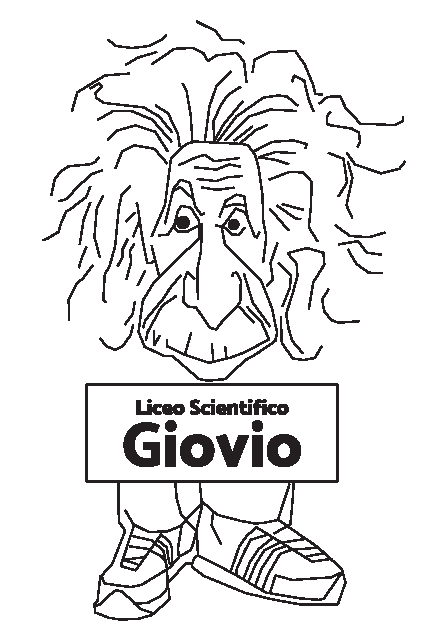
\includegraphics[width=0.7\textwidth]{../.common/Einstein_Logo}
  \label{fig:Einstein_Logo}
\end{figure}


\pagebreak
\tableofcontents

% \pagebreak
% % LTeX: language=it

\section{Piano cartesiano}

% \pagebreak
% % LTeX: language=it

\section{Equazioni e disequazioni con moduli e radici irrazionali}
% % LTeX: language=it

\section{Funzioni}
% % LTeX: language=it

\section{Successioni numeriche}
% % LTeX: language=it

\section{Piano cartesiano (coniche)}

\pagebreak
% LTeX: language=it

\section{Goniometria}

\subsection{Funzioni goniometriche}

\subsubsection*{Addizione}

\begin{itemize}
    \item $\sin(\alpha+\beta)=\sin(\alpha)\cos(\beta)+\cos(\alpha)\sin(\beta)$
    \item $\cos(\alpha+\beta)=\cos(\alpha)\cos(\beta)-\sin(\alpha)\sin(\beta)$
    \item $\tan(\alpha+\beta)=\frac{\tan(\alpha)+\tan(\beta)}{1-\tan(\alpha)\tan(\beta)}$
\end{itemize}

\subsubsection*{Sottrazione}

\begin{itemize}
    \item $\sin(\alpha-\beta)=\sin(\alpha)\cos(\beta)-\cos(\alpha)\sin(\beta)$
    \item $\cos(\alpha-\beta)=\cos(\alpha)\cos(\beta)+\sin(\alpha)\sin(\beta)$
    \item $\tan(\alpha-\beta)=\frac{\tan(\alpha)-\tan(\beta)}{1+\tan(\alpha)\tan(\beta)}$
\end{itemize}

\subsubsection*{Duplicazione}

\begin{itemize}
    \item $\sin(2\alpha)=2\sin(\alpha)\cos(\alpha)$
    \item $\cos(2\alpha)=\cos^2(\alpha)-\sin^2(\alpha)$
    \item $\tan(2\alpha)=2\tan(\alpha)\frac{1-\tan^2(\alpha)}{1+\tan^2(\alpha)}$
\end{itemize}

\subsubsection*{Bisezione}

\begin{itemize}
    \item $\sin(\frac{\alpha}{2})=\sqrt{\frac{1-\cos(\alpha)}{2}}$
    \item $\cos(\frac{\alpha}{2})=\sqrt{\frac{1+\cos(\alpha)}{2}}$
    \item $\tan(\frac{\alpha}{2})=\frac{\sqrt{1-\cos(\alpha)}}{\sqrt{1+\cos(\alpha)}}=\frac{\sin(\alpha)}{1+\cos(\alpha)}=\frac{1-\cos(\alpha)}{1+\cos(\alpha)}$
\end{itemize}

\subsubsection*{Parametriche}

\begin{itemize}
    \item $\sin(\alpha)=\frac{2\tan(\frac{\alpha}{2})}{1+\tan^2(\frac{\alpha}{2})}$
    \item $\cos(\alpha)=\frac{1-\tan^2(\frac{\alpha}{2})}{1+\tan^2(\frac{\alpha}{2})}$
\end{itemize}

\subsubsection*{Esistono anche}

\begin{itemize}
    \item $\sin^2(\alpha)=\frac{1-\cos(2\alpha)}{2}$
    \item $\cos^2(\alpha)=\frac{1+\cos(2\alpha)}{2}$
\end{itemize}

Ogni formula contenente la tangente ha le sue condizioni di esistenza.
In generale essendo $\tan(\alpha)=\frac{\sin(\alpha)}{\cos(\alpha)}$ si ha che $\tan(\alpha)$ esiste se $\cos(\alpha)\neq0$, ovvero se $\alpha\neq K\pi$ con $K \in Z$.
% LTeX: language=it

\section{Trigonometria}
% LTeX: language=it

\section{Esponenziali e logaritmi}
% % LTeX: language=it

\section{Probabilità}
% % LTeX: language=it

\section{Geometria analitica nello spazio}

% \pagebreak
% % LTeX: language=it

\section{Limiti di funzioni}

\subsection{Limiti notevoli}

\subsubsection*{Goniometrici}

\begin{itemize}
    \item $\lim_{x\to0}\frac{\sin(x)}{x}=1$
    \item $\lim_{x\to0}\frac{1-\cos(x)}{x}=0$
    \item $\lim_{x\to0}\frac{1-\cos(x)}{x^2}=\frac{1}{2}$
\end{itemize}

\subsubsection*{Esponenziali e logaritmici}

\begin{itemize}
    \item $\lim_{x\to\infty}(1+\frac{1}{x})^x=e$
    \item $\lim_{x\to0}\frac{a^x-1}{x}=\ln{a}$ con $a>0$ e $a \neq 1$
    \item $\lim_{x\to0}\frac{\log_{a}(1+x)}{x}=\log_{a}(e)$
    \item $\lim_{x\to0}(1+x)^{\frac{1}{x}}=e$
    \item $\lim_{x\to0}\frac{(1+x)^k-1}{x}=k$ con $k \in R$
\end{itemize}
% % LTeX: language=it

\section{Continuità di una funzione}
% % LTeX: language=it

\section{Asintoti}
% % LTeX: language=it

\section{Derivate}
% % LTeX: language=it

\section{Massimi, minimi e flessi}
% % LTeX: language=it

\section{Studio di funzione}
% % LTeX: language=it

\section{Teoremi di calcolo differenziale}
% % LTeX: language=it

\section{Integrali}

\end{document}